\documentclass[12pt]{report}

\usepackage[top=3cm,bottom=3cm,left=3cm,right=3cm]{geometry}
\usepackage{graphicx}
\usepackage{float}
\usepackage{setspace}
\usepackage{fancyhdr}

\setlength{\parindent}{0pt}
\onehalfspacing

\pagestyle{fancy}
\fancyhf{}
\fancyfoot[C]{\thepage}
\renewcommand{\headrulewidth}{0pt}

\begin{document}

\thispagestyle{empty}
\begin{center}
    \vspace*{1.2cm}

    {\Large\textbf{A Report on CyberSecurity, Cryptography and\\
    Network Defense Suite}}\\[1.2cm]

    {\itshape A report submitted in partial fulfillment of the requirements\\
    for the award of the degree of}\\[2.1cm]

    {\large\textbf{by}}\\[0.7cm]

    \begin{tabular}{c c}
        \textbf{K.VISHNU VARDHAN REDDY} & \textbf{2420030063}
    \end{tabular}\\[1.2cm]

    \textbf{Dr.Jagan Mohan Reddy D}

    \vfill

    
\includegraphics[width=0.34\textwidth]{images/logo.png}\\[0.9cm]

    \textbf{KONERU LAKSHMAIAH EDUCATION FOUNDATION, BOWRAMPET}\\[0.45cm]
    \textbf{Hyderabad-500043, Telangana, India}\\[0.45cm]
    2026

    \vspace*{0.4cm}
\end{center}
\clearpage

\chapter*{About the Project}

The \textbf{CyberSecurity, Cryptography and Network Defense Suite} is an educational project developed for Active Learning Management Project--2 (ALM-2). It combines three independent security projects in one unified React and Vite dashboard. The backend services are developed using Python and Flask.

The first project, \textbf{CryptoVault}, demonstrates public-key cryptography, RSA encryption, digital signatures, X.509 certificates, Diffie--Hellman key exchange, and Elgamal signatures. The second project, \textbf{SecureTunnel}, explains TLS, SSH, and IPsec secure communication. The third project, \textbf{Sentinel}, demonstrates firewall rules, bastion-host protection, intrusion detection, and statistical anomaly detection.

The project converts cybersecurity theory into an interactive practical demonstration. All three modules can be opened from one dashboard, while each backend operates independently on its own port.

\begin{figure}[H]
    \centering
    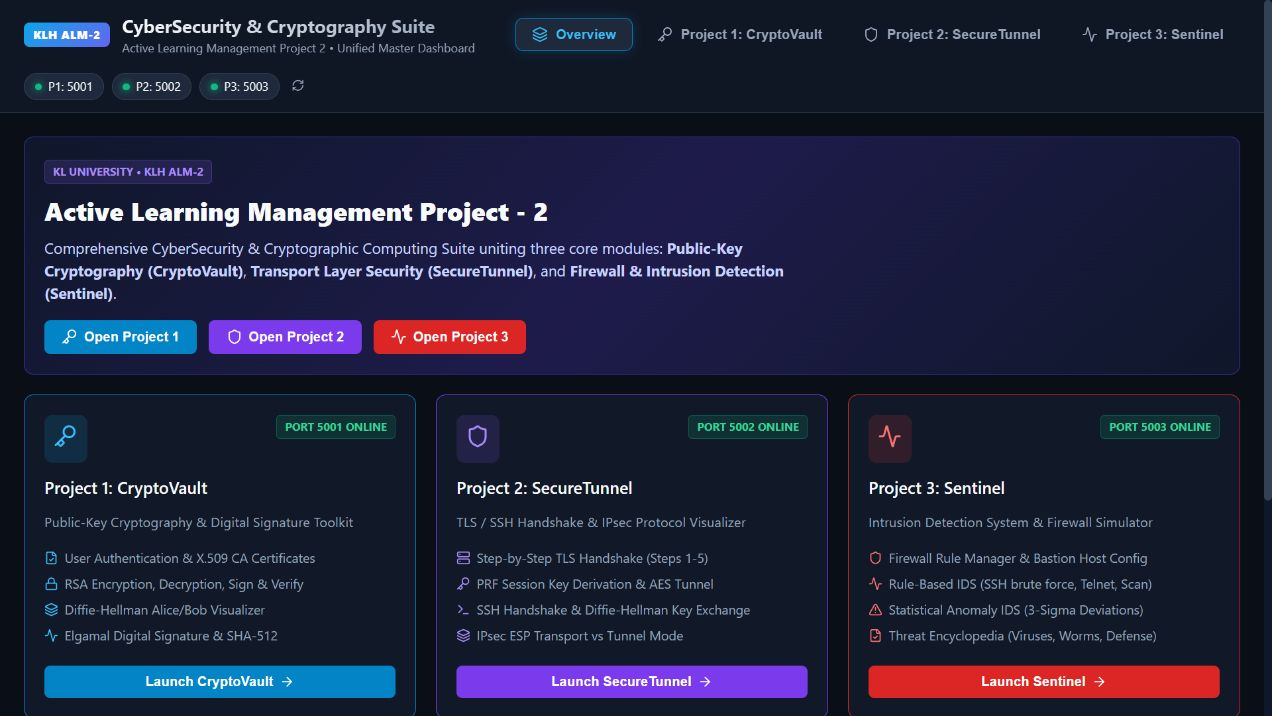
\includegraphics[width=\textwidth]{images/dashboard-overview.jpg}
    \caption{Unified ALM-2 CyberSecurity Dashboard}
\end{figure}

The dashboard displays the live status of CryptoVault, SecureTunnel, and Sentinel and provides direct navigation to each module.

\clearpage

\chapter*{Project 1: CryptoVault}

\begin{figure}[H]
    \centering
    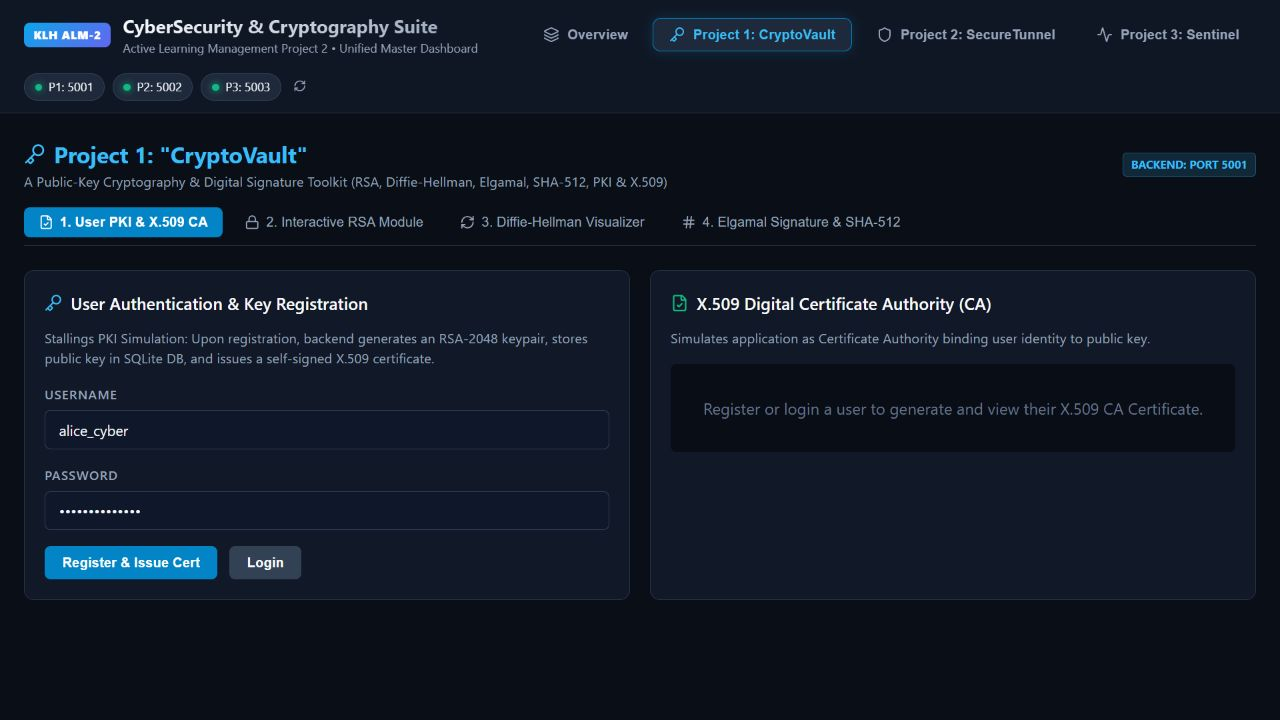
\includegraphics[width=\textwidth]{images/project1-cryptovault.jpg}
    \caption{CryptoVault Cryptography and PKI Module}
\end{figure}

CryptoVault is used to demonstrate user registration, RSA-2048 key generation, X.509 certificates, RSA encryption and signatures, Diffie--Hellman key agreement, and Elgamal signatures with SHA-512.

\section*{Main Features}
\begin{itemize}
    \item \textbf{User Authentication and PKI:} Registers users, creates key pairs, and issues X.509 certificates.
    \item \textbf{RSA Module:} Performs RSA-OAEP encryption and decryption and RSA-PSS signing and verification.
    \item \textbf{Diffie--Hellman:} Shows how two users generate the same shared secret over an insecure channel.
    \item \textbf{Elgamal and SHA-512:} Hashes messages and creates verifiable Elgamal digital signatures.
\end{itemize}

\section*{Security Concepts Demonstrated}
This module explains confidentiality, integrity, authentication, non-repudiation, digital certificates, and secure key agreement.

\clearpage

\chapter*{Project 2: SecureTunnel}

\begin{figure}[H]
    \centering
    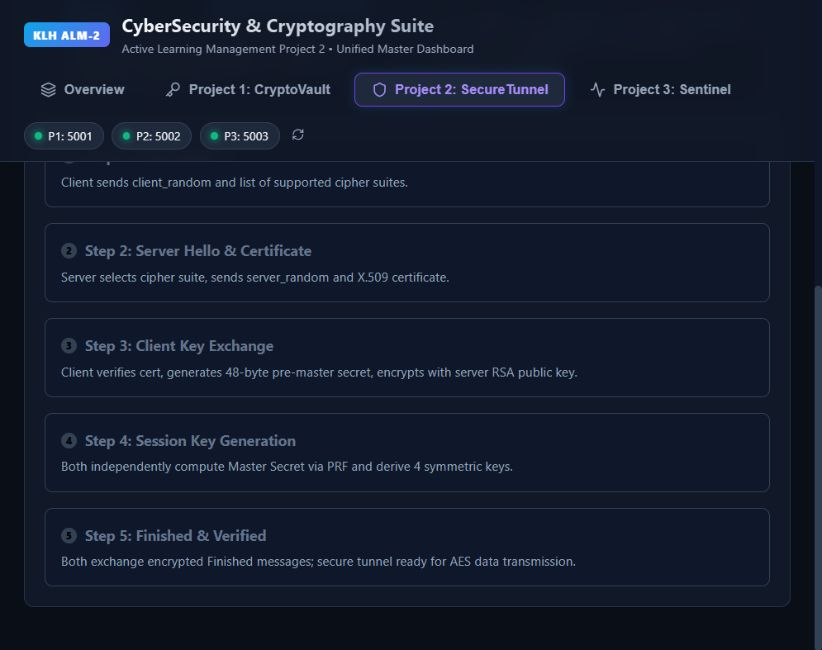
\includegraphics[width=\textwidth]{images/project2-securetunnel.jpg}
    \caption{SecureTunnel TLS, SSH and IPsec Module}
\end{figure}

SecureTunnel visually explains how secure communication channels are established over an untrusted network. It demonstrates TLS, SSH, encrypted data transfer, and IPsec ESP packet protection.

\section*{Main Features}
\begin{itemize}
    \item \textbf{TLS Handshake:} Demonstrates Client Hello, Server Hello, certificate exchange, key generation, and Finished verification.
    \item \textbf{Encrypted Data Transfer:} Protects application data using an AES-GCM symmetric session key.
    \item \textbf{SSH Connection:} Explains key exchange, server authentication, user authentication, and secure shell creation.
    \item \textbf{IPsec ESP:} Compares transport mode with tunnel mode and displays protected packet sections.
\end{itemize}

\section*{Security Concepts Demonstrated}
This module explains encryption, authentication, session-key derivation, integrity checking, and secure tunnelling for web, remote-access, and network traffic.

\clearpage

\chapter*{Project 3: Sentinel}

\begin{figure}[H]
    \centering
    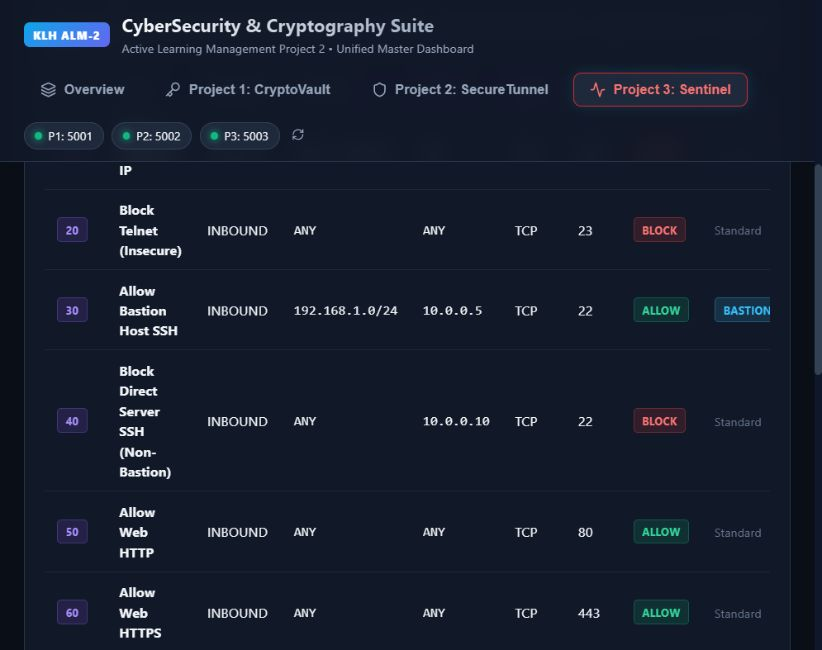
\includegraphics[width=\textwidth]{images/project3-sentinel.jpg}
    \caption{Sentinel Firewall and Intrusion Detection Module}
\end{figure}

Sentinel demonstrates a priority-based firewall, a protected bastion host, live packet inspection, and intrusion detection. It combines known attack rules with statistical traffic analysis.

\section*{Main Features}
\begin{itemize}
    \item \textbf{Firewall Rules:} Allows or blocks packets using addresses, protocol, port, action, and priority.
    \item \textbf{Default-Deny Policy:} Blocks traffic that does not match an approved allow rule.
    \item \textbf{Bastion Host:} Provides a controlled administrative gateway to the protected network.
    \item \textbf{Rule-Based IDS:} Detects SSH brute force, Telnet traffic, and port scanning.
    \item \textbf{Anomaly Detection:} Uses a three-sigma threshold to identify unusual increases in traffic.
    \item \textbf{Threat Encyclopedia:} Provides information about viruses, worms, attacks, and defenses.
\end{itemize}

\section*{Security Concepts Demonstrated}
This module explains access control, defense in depth, packet filtering, network monitoring, and the difference between signature-based and anomaly-based intrusion detection.

\end{document}
